\documentclass{standalone}
\usepackage{tikz}
\usetikzlibrary{patterns, positioning}

\begin{document}
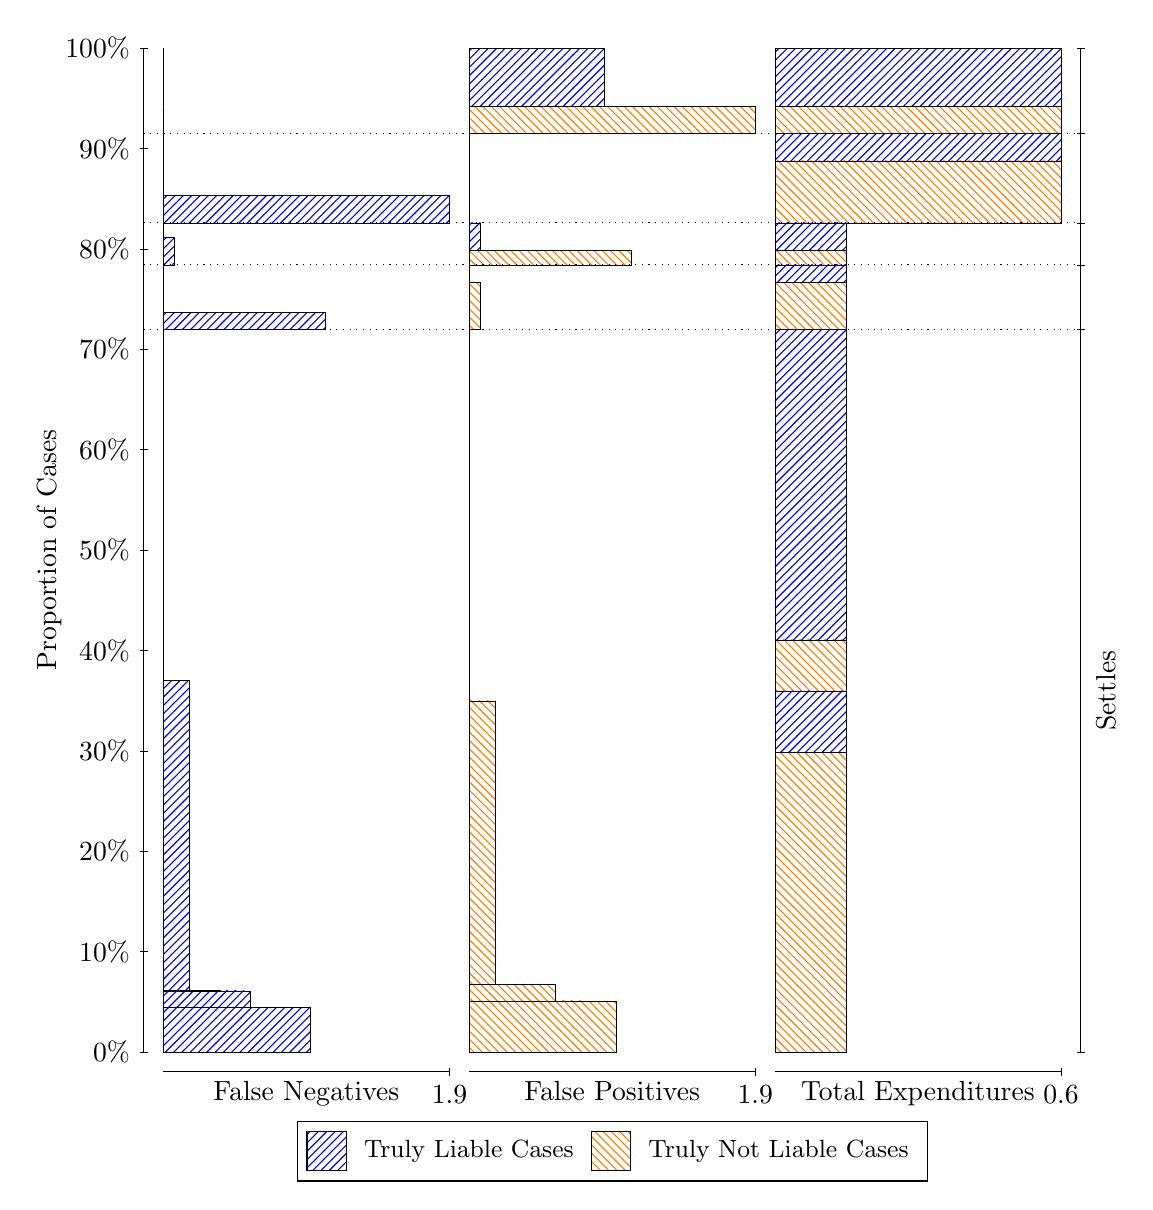
\begin{tikzpicture}
\draw[black, very thin] (1.5,1.75) -- (1.5,14.5);
\node[rotate=90, anchor=center] at (0.3, 8.125) {Proportion of Cases};
\draw[black, very thin] (1.45,1.75) -- (1.55,1.75);
\node[anchor=east] at (1.45, 1.75) {0\%};
\draw[black, very thin] (1.45,3.025) -- (1.55,3.025);
\node[anchor=east] at (1.45, 3.025) {10\%};
\draw[black, very thin] (1.45,4.3) -- (1.55,4.3);
\node[anchor=east] at (1.45, 4.3) {20\%};
\draw[black, very thin] (1.45,5.575) -- (1.55,5.575);
\node[anchor=east] at (1.45, 5.575) {30\%};
\draw[black, very thin] (1.45,6.85) -- (1.55,6.85);
\node[anchor=east] at (1.45, 6.85) {40\%};
\draw[black, very thin] (1.45,8.125) -- (1.55,8.125);
\node[anchor=east] at (1.45, 8.125) {50\%};
\draw[black, very thin] (1.45,9.4) -- (1.55,9.4);
\node[anchor=east] at (1.45, 9.4) {60\%};
\draw[black, very thin] (1.45,10.675) -- (1.55,10.675);
\node[anchor=east] at (1.45, 10.675) {70\%};
\draw[black, very thin] (1.45,11.95) -- (1.55,11.95);
\node[anchor=east] at (1.45, 11.95) {80\%};
\draw[black, very thin] (1.45,13.225) -- (1.55,13.225);
\node[anchor=east] at (1.45, 13.225) {90\%};
\draw[black, very thin] (1.45,14.5) -- (1.55,14.5);
\node[anchor=east] at (1.45, 14.5) {100\%};

\draw[black, very thin] (13.4,1.75) -- (13.4,14.5);
\draw[black, very thin] (13.35,1.75) -- (13.45,1.75);
\node[anchor=west] at (13.35, 1.75) {};
\draw[black, very thin] (13.35,10.923) -- (13.45,10.923);
\node[anchor=west] at (13.35, 10.923) {};
\draw[black, very thin] (13.35,11.746) -- (13.45,11.746);
\node[anchor=west] at (13.35, 11.746) {};
\draw[black, very thin] (13.35,12.28) -- (13.45,12.28);
\node[anchor=west] at (13.35, 12.28) {};
\draw[black, very thin] (13.35,13.413) -- (13.45,13.413);
\node[anchor=west] at (13.35, 13.413) {};
\draw[black, very thin] (13.35,14.5) -- (13.45,14.5);
\node[anchor=west] at (13.35, 14.5) {};

\draw[black, very thin, pattern color=blue, pattern=north east lines] (1.75,1.75) rectangle (3.6145,2.3208);
\draw[black, very thin, pattern color=blue, pattern=north east lines] (1.75,2.3208) rectangle (2.8496,2.5264);
\draw[black, very thin, pattern color=blue, pattern=north east lines] (1.75,2.5264) rectangle (2.6583,2.5268);
\draw[black, very thin, pattern color=blue, pattern=north east lines] (1.75,2.5268) rectangle (2.4671,2.5273);
\draw[black, very thin, pattern color=blue, pattern=north east lines] (1.75,2.5273) rectangle (2.2759,2.5278);
\draw[black, very thin, pattern color=blue, pattern=north east lines] (1.75,2.5278) rectangle (2.0846,6.4654);
\draw[black, very thin, pattern color=orange, pattern=north west lines] (1.75,6.4654) rectangle (1.75,10.923);
\draw[black, very thin, pattern color=blue, pattern=north east lines] (1.75,10.923) rectangle (3.8057,11.143);
\draw[black, very thin, pattern color=orange, pattern=north west lines] (1.75,11.143) rectangle (1.75,11.746);
\draw[black, very thin, pattern color=blue, pattern=north east lines] (1.75,11.746) rectangle (1.8934,12.098);
\draw[black, very thin, pattern color=orange, pattern=north west lines] (1.75,12.098) rectangle (1.75,12.28);
\draw[black, very thin, pattern color=blue, pattern=north east lines] (1.75,12.28) rectangle (5.3833,12.626);
\draw[black, very thin, pattern color=orange, pattern=north west lines] (1.75,12.626) rectangle (1.75,13.413);
\draw[black, very thin, pattern color=orange, pattern=north west lines] (1.75,13.413) rectangle (1.75,13.758);
\draw[black, very thin, pattern color=blue, pattern=north east lines] (1.75,13.758) rectangle (1.75,14.5);
\draw[black, very thin, pattern color=orange, pattern=north west lines] (5.6333,1.75) rectangle (7.4978,2.3958);
\draw[black, very thin, pattern color=orange, pattern=north west lines] (5.6333,2.3958) rectangle (7.3066,2.3968);
\draw[black, very thin, pattern color=orange, pattern=north west lines] (5.6333,2.3968) rectangle (7.1154,2.3977);
\draw[black, very thin, pattern color=orange, pattern=north west lines] (5.6333,2.3977) rectangle (6.9241,2.3986);
\draw[black, very thin, pattern color=orange, pattern=north west lines] (5.6333,2.3986) rectangle (6.7329,2.6061);
\draw[black, very thin, pattern color=orange, pattern=north west lines] (5.6333,2.6061) rectangle (5.968,6.2078);
\draw[black, very thin, pattern color=blue, pattern=north east lines] (5.6333,6.2078) rectangle (5.6333,10.923);
\draw[black, very thin, pattern color=orange, pattern=north west lines] (5.6333,10.923) rectangle (5.7768,11.526);
\draw[black, very thin, pattern color=blue, pattern=north east lines] (5.6333,11.526) rectangle (5.6333,11.746);
\draw[black, very thin, pattern color=orange, pattern=north west lines] (5.6333,11.746) rectangle (7.689,11.928);
\draw[black, very thin, pattern color=blue, pattern=north east lines] (5.6333,11.928) rectangle (5.7768,12.28);
\draw[black, very thin, pattern color=orange, pattern=north west lines] (5.6333,12.28) rectangle (5.6333,13.067);
\draw[black, very thin, pattern color=blue, pattern=north east lines] (5.6333,13.067) rectangle (5.6333,13.413);
\draw[black, very thin, pattern color=orange, pattern=north west lines] (5.6333,13.413) rectangle (9.2667,13.758);
\draw[black, very thin, pattern color=blue, pattern=north east lines] (5.6333,13.758) rectangle (7.3544,14.5);
\draw[black, very thin, pattern color=orange, pattern=north west lines] (9.5167,1.75) rectangle (10.425,5.5592);
\draw[black, very thin, pattern color=blue, pattern=north east lines] (9.5167,5.5592) rectangle (10.425,6.3355);
\draw[black, very thin, pattern color=orange, pattern=north west lines] (9.5167,6.3355) rectangle (10.425,6.9842);
\draw[black, very thin, pattern color=blue, pattern=north east lines] (9.5167,6.9842) rectangle (10.425,10.923);
\draw[black, very thin, pattern color=orange, pattern=north west lines] (9.5167,10.923) rectangle (10.425,11.526);
\draw[black, very thin, pattern color=blue, pattern=north east lines] (9.5167,11.526) rectangle (10.425,11.746);
\draw[black, very thin, pattern color=orange, pattern=north west lines] (9.5167,11.746) rectangle (10.425,11.928);
\draw[black, very thin, pattern color=blue, pattern=north east lines] (9.5167,11.928) rectangle (10.425,12.28);
\draw[black, very thin, pattern color=orange, pattern=north west lines] (9.5167,12.28) rectangle (13.15,13.067);
\draw[black, very thin, pattern color=blue, pattern=north east lines] (9.5167,13.067) rectangle (13.15,13.413);
\draw[black, very thin, pattern color=orange, pattern=north west lines] (9.5167,13.413) rectangle (13.15,13.758);
\draw[black, very thin, pattern color=blue, pattern=north east lines] (9.5167,13.758) rectangle (13.15,14.5);
\draw[black, dotted] (1.5,10.923) -- (13.4,10.923);
\draw[black, dotted] (1.5,11.746) -- (13.4,11.746);
\draw[black, dotted] (1.5,12.28) -- (13.4,12.28);
\draw[black, dotted] (1.5,13.413) -- (13.4,13.413);
\draw[black, very thin] (1.75,1.5) -- (5.3833,1.5);
\node[anchor=north] at (3.5667, 1.5) {False Negatives};
\draw[black, very thin] (5.3833,1.45) -- (5.3833,1.55);
\node[anchor=north] at (5.3833, 1.45) {1.9};

\draw[black, very thin] (5.6333,1.5) -- (9.2667,1.5);
\node[anchor=north] at (7.45, 1.5) {False Positives};
\draw[black, very thin] (9.2667,1.45) -- (9.2667,1.55);
\node[anchor=north] at (9.2667, 1.45) {1.9};

\draw[black, very thin] (9.5167,1.5) -- (13.15,1.5);
\node[anchor=north] at (11.333, 1.5) {Total Expenditures};
\draw[black, very thin] (13.15,1.45) -- (13.15,1.55);
\node[anchor=north] at (13.15, 1.45) {0.6};

\node[black, centered, rotate=90] at (13.72, 6.3366) {Settles};





\draw (7.449999999999999,1.5) node[draw=none] (baseCoordinate) {};
\begin{scope}[align=center]
        \matrix[scale=0.5, draw=black, below=0.5cm of baseCoordinate, nodes={draw}, column sep=0.1cm]{
            \node[rectangle, draw, minimum width=0.5cm, minimum height=0.5cm, pattern=north east lines, pattern color=blue] {}; &
            \node[draw=none, font=\small] (B) {Truly Liable Cases}; &
            \node[rectangle, draw, minimum width=0.5cm, minimum height=0.5cm, pattern=north west lines, pattern color=orange] {}; &
            \node[draw=none, font=\small] (B) {Truly Not Liable Cases}; \\
            };
\end{scope}

\end{tikzpicture}
\end{document}